Como lo explicado en la sección precedente, la aplicación del cliente inicia mostrando una sucesión de pantallas para conectarse al servidor y crear o unirse a una partida. Cada \textit{input} de teclado o mouse que se detecta por parte de un jugador es procesado en caso de que sea el turno del mismo, no se le haya acabado el tiempo, la partida no haya terminado, y el jugador no haya perdido. La acción que debe realizarse en base al \textit{input} del jugador se decide de acuerdo al estado en el que se encuentre el gusano, el cual responde y dicha respuesta es enviada al servidor. Se utilizó el patrón de diseño \textit{State} para modelar todos los posibles estados del gusano. El servidor es el que tiene la lógica del juego, entonces siempre se envía al cliente el estado en el que se encuentran los gusanos. Cada estado tiene asociada una animación y en ciertos casos también un sonido.\\
\indent Las texturas utilizadas en las animaciones y los sonidos (tanto los efectos de sonido como la música de fondo), se cargan en memoria una única vez al comienzo de la partida a fin de no comprometer la \textit{performance} de la aplicación, ya que el proceso de animar se realiza permanentemente, y cargar las diferentes texturas una y otra vez no sería eficiente, al igual que en lo que respecta a los sonidos.\\
\indent Para las diferentes armas que ofrece el juego se realizó otro patrón \textit{State}, de modo que cada vez que hay un disparo, cada arma sabe cómo responder.

\subsection{Desarrollo del juego}
El cliente tiene 3 threads:

\begin{itemize}
    \item El principal (renderer).
    \item El input worker.
    \item El output worker.
\end{itemize}


\subsubsection{Renderer}

Este thread es el encargado de dibujar el juego en la pantalla. Si bien maneja algunas animaciones \textit{client side},
mayormente dibuja el \'ultimo \textit{snapshot} recibido del modelo. Es importante que este thread no se bloquee en ninguna
operaci\'on ya que dar\'ia la sensaci\'on de que el juego no responde. Es por esto que de no haber recibido un
\textit{snapshot} nuevo, de todas formas continua ejecut\'andose y dibujando el \'ultimo recibido (adem\'as de continuar
actualizando las animaciones est\'eticas).

Otra tarea es la de obtener los eventos de \textit{SDL} para procesarlos y actualizar animaciones. Esto no se realiza
en un \textit{thread} independiente porque no es necesario ya que un ser humano no tiene la velocidad de generar demasiados
eventos en una iteración de forma que se pudiera demorar proces\'andolos. Esto resulta una ventaja porque de esta
forma no es necesaria la utilizaci\'on de \textit{threads} (y \textit{mutex}) en el \textit{render loop}, minimizando los posibles errores
y la complejidad del mismo.


\subsubsection{Input worker}

Este \textit{thread} obtiene de la conexi\'on con el servidor los nuevos \textit{snapshots}. De forma similar a como trabaja el servidor,
este \textit{thread} almacena los snapshots en un \texttt{DoubleBuffer}, con la diferencia de que el \texttt{Renderer} no
se bloquea esperando un \texttt{swap}, sino que siempre obtiene una copia (aunque sea una ya leída previamente).


\subsubsection{Output worker}

El cliente debe enviar las acciones del mismo al servidor mediante el \textit{socket}. Para evitar bloquearse en un \texttt{send},
esta tarea es realizada por un \textit{thread}. La comunicaci\'on entre este \textit{thread} y el \textit{renderer} se realiza mediante un
\texttt{Stream}. El \textit{renderer} hace \texttt{push} y este \textit{thread} hace un \texttt{pop} bloqueante para evitar un \textit{busy wait}.
Cada acci\'on es luego serializada y enviada al servidor.


En la figura \ref{im:comunicacion} muestra la comunicaci\'on entre un cliente y el servidor. Cada flecha vertical representa un \textit{thread}
en el proceso en el cual se origina, mientras que las flechas horizontales indican comunicaci\'on de alguna forma:

\begin{figure}[H]
	\centering
	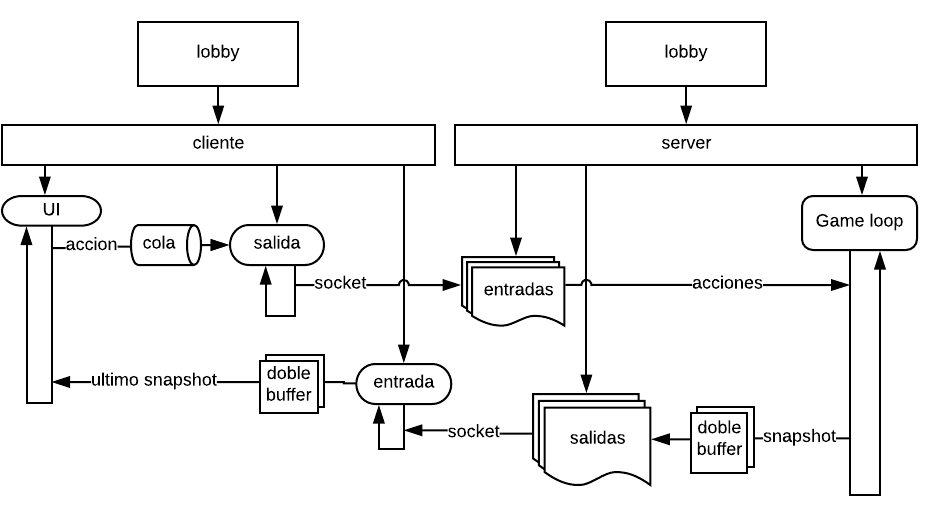
\includegraphics[width=\textwidth,height=\textheight,keepaspectratio]{gameCommunication.png}
	\caption{Comunicación entre cliente y servidor}
	\label{im:comunicacion}
\end{figure}

\subsection{Clases}

Primero se describen las clases que son utilizadas tanto por el cliente como por el servidor.

\begin{itemize}
	\item \textbf{\textit{Direction}}: clase \textit{enum} que indica la dirección del gusano (derecha o izquierda).
	
	\item \textbf{\textit{DoubleBuffer}}: se utiliza para enviar (en el servidor), y recibir (en el cliente), los \textit{snapshots} con la información del estado del juego.
	
	\item \textbf{\textit{EnumClassHash}}: es una estructura que define el operador \textit{()} para tipos enumerativos.
	
	\item \textbf{\textit{Exception}}: se adaptó la clase \textit{OSError}, usando funciones estándar de C++11, para hacer una clase genérica de excepción, la cual recibe el formato de la cadena de texto y los argumentos para completar el formato.
	
	\item \textbf{\textit{Stream}}: es una clase \textit{template} que encapsula una cola que puede ser utilizada como bloqueante. El parámetro del \textit{template} es el mensaje que se va a enviar por la misma. Sus métodos son \textit{push}, \textit{pop} y \textit{close}, que impide el uso de la cola ya que al hacer \textit{pop} lanza una excepción. Tiene sobrecargados los operadores $<<$ y $>>$ para hacer \textit{push} y \textit{pop} de manera bloqueante respectivamente.
	
	\item \textbf{\textit{StateID}}: clase \textit{enum} que posee todos los estados del gusano.
	
	\item \textbf{\textit{WeaponID}}: clase \textit{enum} que posee todos los estados de las armas.
	
	\item \textbf{\textit{PlayerInput}}: clase \textit{enum} que posee todos los \textit{inputs} que puede generar el usuario.
	
	\item \textbf{\textit{PlayerMsg}}: es una estructura que posee un \textit{PlayerInput} y una posición (cuando se produce un evento de click con el mouse en la utilización de un arma que lo requiera) y que envía el cliente al servidor.
	
	\item \textbf{\textit{GameStateMsg}}: es una estructura que posee todos los elementos que conforman el estado del juego en un momento dado, el cual el servidor envía a los clientes. Sus métodos son \textit{serialize}, y \textit{deserialize}, que se encargan de procesar los datos para enviarlos y recibirlos adecuadamente de una forma portable.
	
	\item \textbf{\textit{LevelInfo}}: es una estructura que posee la información correspondiente a un nivel (\textit{id}, nombre y cantidad de jugadores). La envía el servidor al cliente.
	
	\item \textbf{\textit{GameInfo}}: es una estructura que posee la información correspondiente a una partida ya creada (\textit{id} de la partida, \textit{id} y nombre del nivel asociado a la misma, cantidad actual de jugadores y cantidad total de jugadores necesaria para comenzar la partida). La envía el servidor al cliente.
	
	\item \textbf{\textit{Event}}: es una clase \textit{enum} que posee todos los eventos que pueden suceder en el juego y fuera del mismo, tanto en el cliente como en el servidor.
	
	\item \textbf{\textit{Subject}}: es una clase que posee un \textit{set} de punteros a \textit{Observer}. Sus métodos son \textit{addObserver} y \textit{removeObserver} para agregar o quitar observadores al sujeto, y \textit{notify}, el cual recibe a dicho sujeto como referencia y el evento que este quiere notificar.
	
	\item \textbf{\textit{Observer}}: es una interfaz cuyo único método es \textit{onNotify}, que recibe un \textit{Subject} como referencia y un \textit{Event} que este notifica.
	
	\item \textbf{\textit{Point}}: es una clase \textit{template} que define un punto de coordenadas \textit{(x, y)} del tipo numérico indicado en el \textit{template} y define las operaciones de suma, resta, multiplicación, división y los operadores $==$ y  $!=$, además de la distancia entre dos puntos.
	
	\item \textbf{\textit{Socket}}: implementación según el paradigma de objetos socket. Es una implementación para que las clases hijas (\emph{ServerSocket}, \emph{CommunicationSocket} y \emph{ClientSocket}) implementen y se utilicen de forma RAII la comunicación entre equipos. En la figura \ref{im:socket} puede verse un diagrama de clase de estas clases mencionadas. Sabe como destruirse y también como construirse por movimiento (también asignación por movimiento). Sus métodos son \textit{close}, que cierra el \textit{file descriptor} y \textit{shutdown}, que cierra la comunicación bidireccionalmente. El método close es protegido y solo puede usarse internamente en alguna de las hijas. También se usa internamente en el destructor.
	
	\item \textbf{\textit{Protocol}}: es una clase \textit{template} donde el parámetro del \textit{template} es el tipo de \textit{socket} que utilizará. Establece un protocolo de comunicación entre cliente y servidor. Tiene sobrecargados los operadores $>>$ y $<<$ para diversos tipos de datos, y los métodos \textit{getSocket}, que devuelve por movimiento el \textit{socket} dejando inutilizado el protocolo, y \textit{stopCommunication}, que para la comunicación del \textit{socket} mediante un \textit{shutdown}.
	
	\item \textbf{\textit{Thread}}: es una clase abstracta que encapsula un hilo. Sus métodos son \textit{start} para lanzar el hilo y \textit{join} para terminarlo. Todas las clases que hereden de esta deben implementar los métodos \textit{run}, donde se define lo que se desea que el hilo haga, y \textit{stop}, para terminar su ejecución de manera ordenada si es necesario.
	
	\item \textbf{\textit{GirderData}}: es una estructura utilizada en \textit{Stage} para almacenar la información correspondiente a las vigas (largo, alto, ángulo y posición).
	
	\item \textbf{\textit{WormData}}: es una estructura utilizada en \textit{Stage} para almacenar la información correspondiente a los gusanos (vida y posición).
	
	\item \textbf{\textit{Color}}: es una estructura utilizada en \textit{Stage} para almacenar la información correspondiente a un color (sus componentes \textit{r}, \textit{g} y \textit{b}).
	
	\item \textbf{\textit{Stage}}: carga la información de un nivel desde un archivo de configuración en formato \textit{YAML} con el método estático \textit{fromFile} utilizando las funciones estáticas \textit{\_parsePoint}, \textit{\_parseWorm} y \textit{\_parseGirder}, y luego devuelve un \textit{Stage} con los datos ya cargados. Se construye creando un mapa \textit{unordered map} para asociar los nombres de las armas con sus \textit{ids}. El método \textit{getAmmoCounter} devuelve una referencia constante a un mapa donde se almacena la cantidad de municiones que cada jugador dispone de cada arma en el nivel.
\end{itemize}

\begin{figure}[H]
	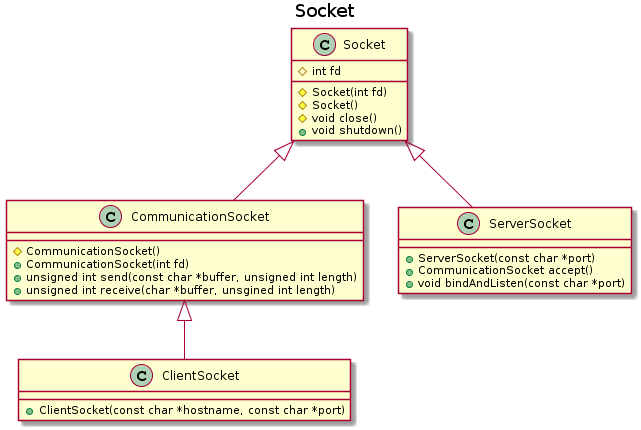
\includegraphics[scale=0.6]{Socket.png}
	\caption{Diagrama de clase de Socket}
	\label{im:socket}
\end{figure}
A continuación se describen las clases propias del cliente:

\begin{itemize}
	\item \textbf{\textit{Window}}: se construye a partir de un ancho y alto fijos o personalizados, e inicia todos los recursos de \textit{SDL} que se utilizarán. Al destruirse llama al método \textit{close}, el cual se encarga de liberar todos los recursos adquiridos. Se destacan los métodos \textit{clear}, que pone la ventana en un color determinado por parámetro o en blanco por defecto, \textit{containsMouse}, que indica si el mouse está contenido en la ventana, \textit{maximize}, que maximiza la ventana, \textit{getRenderer}, que devuelve el renderizador de la ventana, y \textit{render}, que renderiza el contenido de la ventana.
	
	\item \textbf{\textit{Animation}}: se construye a partir de una textura y se encarga de renderizar la misma de acuerdo a un \textit{framrate} de 25 \textit{frames} or segundo en la posición que se le indica. Puede renderizarse en \textit{loop} desde el \textit{frame} incial hasta el último y a continuación el primero nuevamente, en \textit{loop} llegando al final y volviendo al comienzo (indicado con el \textit{flag} \textit{playReversed}), animarse una única vez quedando en el último \textit{frame} (indicado con el \textit{flag} \textit{playOnce}), animarse en sentido inverso (indicado con el \textit{flag} \textit{playInverse} y utilizado para la teletransportación) o puede setearse un \textit{frame} manualmente (para el caso en el que se esté apuntando un arma por ejemplo). La actualización del \textit{frame} que debe renderizarse se hace mediante el método \textit{update}, el cual recibe el tiempo que ha pasado desde el último cambio. Cuando este tiempo acumulado supera el \textit{framrate} se realiza el cambio de \textit{frame}.\\
	\indent Los métodos principales son el ya mencionado \textit{update}, el método \textit{render}, que recibe la posición en donde debe renderizarse, el modo de \textit{flip}, y la cámara del juego que es la que calcula las coordenadas y la muestra en pantalla. Finalmente el método \textit{advanceFrame} es el que se encarga, en base a los \textit{flags} que se encuentren seteados, de establecer el siguiente \textit{frame} que debe ser animado.
	
	\item \textbf{\textit{Camera}}: se construye en base a la ventana donde se renderizará, la relación pixels/metro deseada  y el ancho y alto del área a donde la cámara puede ir. Se destacan los métodos \textit{isMoving} para saber si la cámara está en movimiento a la hora de decidir qué renderizar, \textit{update} que se encarga de actualizar la posición de la cámara, y luego los métodos \textit{draw} y \textit{drawLocal} que dibujan en pantalla una textura o un rectángulo que reciben por parámetro.
	
	\item \textbf{\textit{Texture}}: encapsula la creación y liberación de recursos correspondiente a una textura. Únicamente devuelve el puntero correspondiente a la textura, su alto o su ancho.
	
	\item \textbf{\textit{Font}}: encapsula la creación y liberación de recursos correspondiente a una fuente de texto. Solo devuelve un puntero correspondiente a la fuente.
	
	\item \textbf{\textit{Text}}: se construye a partir de una fuente. Se le setea el texto deseado e internamente crea una textura con el mismo, la cual es renderizada con o sin fondo. El método \textit{render} es el encargado de dibujar el texto en pantalla de acuerdo a una posición y la cámara recibidos por parámetro.

	\item \textbf{\textit{WrapTexture}}: se crea a partir de una textura, un ancho y un alto. Solapa la misma textura o la recorta en base a las dimensiones de la misma y al ancho y al alto especificados. Se destaca el método \textit{render}, que dibuja la textura en pantalla en la posición deseada y el método \textit{render} que hace lo propio pero especificando también un ángulo.
	
	\item \textbf{\textit{Button}}: representa un botón y se crea a partid de una posición, un ancho y un alto. Puede seteársele un mensaje y el color de texto y de fondo. Se destaca el método \textit{inside} que establece a partir de la posición en la que el usuario hizo click recibida por parámetro si esta se encuentra dentro del botón, y \textit{render}, que a partir de una \textit{cámara} recibida por parámetro lo dibuja en pantalla.
	
	\item \textbf{\textit{GameWindow}}: hereda de \textit{Subject}. Es una interfaz para todas las ventanas que posee la aplicación y comunica las acciones realizadas en estas a un observador que será \textit{LobbyAssistant}, que se describirá luego. Se construye a partir de la ventana del juego, una fuente de texto y una cámara. Define una estructura \textit{TextField} que procesa los \textit{inputs} de texto del usuario, y tiene un vector de botones \textit{Button}. Posee los métodos \textit{handleKeyDown} (responde a \textit{inputs} del usuario), \textit{appendCharacter} (responde a \textit{inputs} de texto del usuario), \textit{buttonPressed} (responde en el caso que un usuario presione un botón), y \textit{render} (dibuja todo lo que deba dibujarse en la ventana). Las clases que implementan esta interfaz son:
	\begin{itemize}
		\item \textbf{\textit{ConnectionWindow}}: tiene dos \textit{TextField} donde permite al usuario ingresar la \textit{ip} y el puerto del servidor al que desea conectarse y un botón que al presionarlo crea la conexión.
		\item \textbf{\textit{SelecActionWindow}}: tiene dos botones con los cuales permite al usuario elegir entre crear una partida o unirse a una existente.
		\item \textbf{\textit{CreateGameWindow}}: permite crear una partida. Muestra en pantalla un nivel con su nombre y cantidad de jugadores y tiene tres botones, dos para alternar entre los niveles disponibles (anterior y siguiente), y otro para seleccionar el nivel.
		\item \textbf{\textit{JoinGameWindow}}: permite unirse a una partida. Muestra en pantalla una partida con la cantidad de jugadores que hay actualmente en dicha partida y la cantidad de jugadores que debe haber para comenzar. Tiene tres botones, dos para alternar entre las partidas disponibles (anterior y siguiente), y otro para seleccionar la partida.
		\item \textbf{\textit{WaitingPlayersWindow}}: una vez que se seleccionó el nivel a crear o se eligió la partida a unirse, se muestra una pantalla con la cantidad actual de jugadores conectados y la cantidad necesaria para que comience el juego. Cuando esta cantidad es alcanzada, el juego comienza automáticamente.
		\item \textbf{\textit{GameEndWindow}}: al finalizar el juego o el jugador desconectarse, se muestra en pantalla un mensaje haciendo alusión a si ganó o perdió.
	\end{itemize}

	\item \textbf{\textit{ClientGUIInput}}: clase \textit{enum} que posee las acciones que el cliente puede realizar.
	
	\item \textbf{\textit{ServerResponseAction}}: clase \textit{enum} que posee las acciones que puede indicarle el servidor al cliente.
	
	\item \textbf{\textit{ClientGUIMsg}}: es una estructura que posee un \textit{ClientGUIInput} y que utiliza \textit{LobbyAssistant} para comunicar acciones a \textit{CommunicationProtocol}, que serán descriptas luego.
	
	\item \textbf{\textit{ServerResponse}}: es una estructura que posee un \textit{ServerResponseAction} y que utiliza \textit{CommunicationProtocol} para comunicar acciones a \textit{LobbyAssistant}, que serán descriptas luego.

	\item \textbf{\textit{ClientSocket}}: es un socket que hereda de \textit{CommunicationSocket} y tiene la capacidad de realizar una conexión con el servidor, partiendo del dato del \textit{host} y el puerto a donde conectarse. No posee métodos propios, solo su constructor que es donde se realiza la conexión.
	
	\item \textbf{\textit{CommunicationProtocol}}: es un hilo, hereda de la clase \textit{Thread} y se construye a partir de un \textit{ClientSocket} que se utiliza para inicializar un atributo correspondiente a un protocolo \textit{Protocol} y dos \textit{Stream}, uno para recibir mensajes de la interfaz gráfica (\textit{ClientGUIMsg}) y otro para enviar mensajes a la interfaz (\textit{ServerResponse}). El \textit{stream} de mensajes del cliente se utiliza como cola bloqueante ya que el hilo no realiza ninguna acción a menos que el cliente lo requiera. Hace de interfaz entre el servidor y el cliente. Posee atributos públicos que son modificados por los datos provenientes del servidor para luego ser leídos por el cliente, o bien para ser modificados por el cliente y posteriormente enviados al servidor. Posee los métodos \textit{run}, donde espera un mensaje del cliente, \textit{handleClientInput}, donde toma la decisión de qué realizar en base al requerimiento del cliente, y luego métodos correspondientes a las acciones que puede realizar dicho cliente. Estos son: \begin{itemize}
		\item \textit{startCreateGame}: envía el comando correspondiente al servidor y recibe la información de los niveles disponibles.
		
		\item \textit{createGame}: envía el comando correspondiente al servidor y el nivel elegido. Recibe el archivo de configuración del nivel y sus fondos y luego espera el comienzo del juego en \textit{waitGameStart}.
		
		\item \textit{startJoinGame}: envía el comando correspondiente al servidor y recibe las partidas disponibles.
		
		\item \textit{joinGame}: envía el comando correspondiente al servidor, la partida elegida y el nivel que asociado a la partida elegida para luego recibir su archivo de configuración y fondos y luego espera el comienzo del juego en \textit{waitGameStart}.
	\end{itemize}
	También posee el método \textit{waitGameStart}, que espera hasta que la partida alcance el número de jugadores necesario para empezar y avisa al cliente cuando esto sucede. El método \textit{getLevelFiles} se encarga de recibir y guardar en el cliente el archivo de configuración del nivel y sus fondos. Finalmente, el método \textit{getSocket} remueve el \textit{socket} del protocolo mediante \textit{move semantics} (se utiliza para dárselo al juego una vez que este comienza), y le método \textit{stop} para la ejecución del hilo y la comunicación del protocolo para un cierre ordenado.
	
	\item \textbf{\textit{LobbyAssistant}}: hereda de \textit{Observer}, se construye con una ventana \textit{Window} e internamente crea una cámara, una fuente de texto y una ventana de tipo \textit{GameWindow} que cambiará de acuerdo a las acciones del usuario. Se encarga de manejar la lógica de las ventanas iniciales y crea un \textit{CommunicationProtocol} cuando el usuario se conecta al servidor. Posee \textit{streams} de tipo \textit{ClientGUIMsg} para enviar mensajes al hilo del protocolo de comunicación y \textit{ServerResponse} para recibir su respuesta (utilizado como cola no bloqueante), que se procesa en el método \textit{handleServerResponse}. Se destaca el método \textit{run}, donde se reciben \textit{inputs} del usuario, se renderiza la ventana, se realiza un cambio de ventana si es necesario y se procesan respuestas del servidor en caso de haberlas. También se destaca el método \textit{onNotify}, que corresponde a notificaciones de las ventanas y se toma la decisión de qué hacer en base a la interacción del usuario con las mismas. Finalmente, el método \textit{getSocket} devuelve el \textit{socket} obtenido del protocolo de comunicación mediante \textit{move semantics}.
	
	\item \textbf{\textit{Worm}}: esta clase representa al gusano y se construye con un \textit{id} que lo identifica, un \textit{GameTextureManager} y un \textit{SoundEffectManager} ya que de acuerdo a su estado se renderizará con distintas texturas y reproducirá sonidos. Se destacan los métodos \textit{handleKeyDown}, \textit{handleKeyUp} y \textit{mouseButtonDown} para procesar \textit{inputs} del usuario, y \textit{update} que actualiza el estado, la animación, el arma, la explosión asociada a esta si existe y el efecto de sonido si este correspondiera. El método \textit{setState}, que setea su estado con la información proveniente del servidor, y \textit{getAnimation} y \textit{playSoundEffect}, que establecen la textura a renderizar y el sonido a reproducir en base al estado. El método \textit{setWeapon} establece el arma a utilizar y \textit{playWeaponSoundEffect} su efecto de sonido asociado. Finalmente, \textit{startShot} y \textit{endShot} realizan la lógica del disparo de acuerdo a cómo responde el arma.

	\item \textbf{\textit{State}}: representa el estado del gusano. Todos los \textit{inputs} del jugador están representados en métodos (\textit{moveLeft}, \textit{moveRight}, \textit{jump}, \textit{bazooka}, \textit{startShot}, etc.), y cada estado sabrá responder en consecuencia. Se destaca el método que devuelve el \textit{id} del estado. Las clases que implementan esta interfaz son:
	\begin{itemize}
		\item \textbf{\textit{Walk}}.
		\item \textbf{\textit{Still}}.
		\item \textbf{\textit{StartJump}}.
		\item \textbf{\textit{Jump}}.
		\item \textbf{\textit{EndJump}}.
		\item \textbf{\textit{BackFlip}}.
		\item \textbf{\textit{BackFlipping}}.
		\item \textbf{\textit{EndBackFlip}}.
		\item \textbf{\textit{Hit}}.
		\item \textbf{\textit{Die}}.
		\item \textbf{\textit{Dead}}.
		\item \textbf{\textit{Drowning}}.
		\item \textbf{\textit{Falling}}.
		\item \textbf{\textit{Land}}.
		\item \textbf{\textit{Sliding}}.
		\item \textbf{\textit{Teleporting}}.
		\item \textbf{\textit{Teleported}}.
		\item \textbf{\textit{Batting}}.
	\end{itemize}

	\item \textbf{\textit{SoundEffect}}: carga un efecto de sonido para ser reproducido luego. Sus métodos son \textit{getChunk}, que devuelve el puntero al efecto de sonido cargado, y \textit{play}, que lo reproduce una vez o en \textit{loop} de acuerdo al \textit{booleano} que recibe por parámetro.
	
	\item \textbf{\textit{BackgroundMusic}}: carga un archivo de música para utilizarlo como fondo en el juego. Sus métodos son \textit{getMusic}, que devuelve el puntero al archivo de música cargado, y \textit{play}, que lo reproduce en \textit{loop}.
	
	\item \textbf{\textit{TextureManager}}: es un template que permite guardar texturas en un \textit{unordered map} con un \textit{hash} redefinido.
	
	\item \textbf{\textit{SoundEffectManager}}: idéntico funcionamiento que el \textit{TextureManager} salvo que ahora se almacenan efectos de sonido en vez de texturas, y ya no es necesario el renderizador.
	
	\item \textbf{\textit{BackgroundMusicManager}}: idéntico funcionamiento que el \textit{SoundEffectManager} salvo que ahora se almacenan archivos de música de fondo en vez de efectos de sonido.
	
	\item \textbf{\textit{SoundEffectPlayer}}: se construye con un \textit{SoundEffect} obtenido del \textit{SoundEffectManager} y opcionalmente con la duración que se desea del efecto de sonido o si debe actualizarse automáticamente. Sirve de interfaz para la reproducción de efectos de sonido. Se puede establecer mediante un atributo si se desea reproducir el efecto de sonido en \textit{loop}. Sus métodos son \textit{play}, que reproduce el efecto de sonido de acuerdo al valor del atributo \textit{loop}, y \textit{update}, que recibe el tiempo transcurrido desde la última actualización y si no se eligió la actualización automática acumula dicho tiempo. Si este acumulado supera la duración establecida del efecto lo reproduce nuevamente y vuelve el acumulado a cero.
	
	\item \textbf{\textit{BackgroundMusicPlayer}}: se construye a partir de un \textit{BackgroundMusic} obtenido del \textit{BackgroundMusicManager} y reproduce el archivo de música mediante el método \textit{play}.
	
	\item \textbf{\textit{Armory}}: se construye a partir de un \textit{GameTextureManager}, que es un \textit{TextureManager} cuyo \textit{id} es de tipo \textit{GameTextures} (clase \textit{enum} con los \textit{ids} de cada textura utilizada), y también a partir de la cámara del juego y su fuente de texto (ambas referencias). Se encarga de renderizar los íconos de las armas del juego indicando la cantidad de municiones de cada una que le quedan por utilizar al jugador. Posee los métodos \textit{loadWeapons}, donde se cargan en un vector las texturas correspondientes a los íconos de las armas del juego, \textit{update}, que actualiza las municiones de las armas que le quedan al jugador, y \textit{render}, que dibuja en pantalla los íconos con la cantidad de municiones y las teclas para utilizar cada arma (\textit{F1} - \textit{F10}).
	
	\item \textbf{\textit{Wind}}: se construye a partir de un \textit{GameTextureManager} y una cámara, y mediante el método \textit{render} dibuja en pantalla la dirección del viento con un tamaño de acuerdo a la intensidad del mismo.
	
	\item \textbf{\textit{Water}}: se construye a partir de un \textit{GameTextureManager}. Su método \textit{render} dibuja en pantalla la textura del agua, y el método \textit{update} realiza el efecto de animación de la misma.
	
	\item \textbf{\textit{Explosion}}: se construye a partir de un \textit{GameTextureManager} de donde se obtiene la animación necesaria. En el método \textit{render} se renderiza la animación y en el método \textit{update} se actualiza, seteando un \textit{flag} de acuerdo a si esta terminó. Dicho \textit{flag} es devuelto en el método \textit{finished}.
	
	\item \textbf{\textit{Bullet}}: se construye a partir de un \textit{GameTextureManager} de donde se obtiene la animación necesaria de acuerdo al \textit{id} del arma que la disparó, y de un \textit{GameSoundEffectManager} para reproducir el sonido de la explosión. El método \textit{setAngle} setea el ángulo de la bala para actualizar luego la animación en base a este. Con el método \textit{madeImpact} el \textit{Game} le indica a la bala que hizo impacto, por lo que setea un \textit{flag} indicándolo y reproduce el sonido de la explosión. En \textit{render} y \textit{update} se renderiza y actualiza respectivamente la animación de la bala si esta no explotó, o la explosión (de clase \textit{Explosion}, que posee internamente la bala) en caso contrario.
	
	\item \textbf{\textit{Scope}}: se construye a partir de un \textit{GameTextureManager} de donde se obtiene la animación necesaria. El método \textit{setAngle} setea el ángulo en el que apunta el gusano, que luego se utiliza en el método \textit{render} para dibujar la mira en la posición correcta. El método \textit{update} actualiza la animación.
	
	\item \textbf{\textit{PowerBar}}: se construye a partir de un \textit{GameTextureManager} de donde se obtienen las animaciones necesarias. El método \textit{setAngle} setea el ángulo en el que apunta el gusano, que luego se utiliza en el método \textit{render} para dibujar la barra en la posición correcta. El método \textit{update} agrega animaciones para simular el cargado de la barra conforme pasa el tiempo. Los métodos \textit{startShot} y \textit{endShot} determinan cuándo debe renderizarse.
	
	\item \textbf{\textit{Weapon}}: es una clase abstracta que encapsula el comportamiento de las armas. Las clases que heredan de esta se construyen en base a un \textit{GameTextureManager}, el \textit{id} de una textura y el \textit{frame} en que debe setearse (según el ángulo en el que está apuntando el gusano, que luego será alterado por el método \textit{setAngle}). Según el arma, puede poseer mira (\textit{Scope}) y disparar con potencia variable (\textit{PowerBar}). El método \textit{positionSelected} se utiliza para animar el ataque aéreo, y los métodos \textit{startShot} y \textit{endShot} comienzan y terminan la animación de la barra de potencia respectivamente. En el método \textit{update} se actualizan y en el método \textit{render} se dibujan: la mira, la barra de potencia (si estas existen), y la animación del arma. Las clases de armas que heredan de esta son:
	\begin{itemize}
		\item \textbf{\textit{AerialAttack}}.
		\item \textbf{\textit{Banana}}.
		\item \textbf{\textit{BaseballBat}}.
		\item \textbf{\textit{Bazooka}}.
		\item \textbf{\textit{Cluster}}.
		\item \textbf{\textit{Dynamite}}.
		\item \textbf{\textit{Grenade}}.
		\item \textbf{\textit{Holy}}.
		\item \textbf{\textit{Mortar}}.
		\item \textbf{\textit{Teleport}}.
		\item \textbf{\textit{WeaponNone}}.
	\end{itemize}

	\item \textbf{\textit{Game}}: es la clase donde se desarrolla el juego. Uno de los parámetros que recibe al construirse es el número de equipo asociado al jugador, que se utilizará para decidir si se aceptan \textit{inputs} del mismo. Su método \textit{start} tiene el ciclo que se repite hasta que la partida termina o el jugador se desconecta, y en el cual se actualiza el manejo de la cámara mediante \textit{handleCamera}, se actualizan los gusanos, la cámara, el agua, y la/s bala/s si existen mediante \textit{update}, y se renderiza mediante \textit{render}. Se destacan los métodos \textit{loadTextureManager}, \textit{loadSoundManager} y \textit{loadBackgroundManager}, donde se cargan las texturas, efectos de sonido y la música de fondo respectivamente.
\end{itemize}

